\documentclass[11pt, a4paper]{article}
\usepackage[utf8]{inputenc}
\usepackage{amsmath, amssymb}
\usepackage{graphicx}
\usepackage{hyperref}
\usepackage{geometry}
\geometry{margin=1in}

\title{EE 325 Digital Signal Processing \\ Assignment 11: Short-Time Fourier Transform (STFT) and Spectrograms}
\author{PERERA J.D.T. \\ E/21/291}
\date{\today}

\begin{document}
\maketitle

\section{1. Conceptual STFT Discussion}
\subsection{(a) STFT and Non-Stationary Signals}
The standard Fourier Transform implicitly assumes a signal is stationary, extracting its globally sustained frequency content over all time constraints $t \in (-\infty, \infty)$. For non-stationary signals (whose frequency metrics change over time), standard FT provides the average spectrum and completely loses the "when" information. The Short-Time Fourier Transform (STFT) resolves this by utilizing a sliding localizing window function $w(n-m)$, multiplying the signal into short localized segments. Taking the FT of these segments builds a 2D map connecting time, frequency, and magnitude.

\subsection{(b) Time-Frequency Trade-off}
The Heisenberg-Gabor Uncertainty Principle governs STFT resolution ($\Delta t \cdot \Delta f \ge \text{constant}$). 
\begin{itemize}
    \item \textbf{Narrow (Short) Window:} Provides excellent \textbf{time} resolution (can precisely localize when a frequency shift occurs). But standard FT on a short sequence provides terrible \textbf{frequency} resolution (broad, smeared spectral energy).
    \item \textbf{Wide (Long) Window:} Provides excellent \textbf{frequency} resolution (narrow, sharp spectral tone definitions). But it obscures precisely when temporal transitions occurred within the wide window (\textbf{time} smearing).
\end{itemize}

\subsection{(c) Examples Respective to STFT}
A prime example is conversational \textbf{Speech} or a \textbf{Musical Melody}. If one plays the note 'C' and then the note 'G', an ordinary FT only asserts that both 'C' and 'G' frequencies exist in the record. The STFT successfully portrays 'C' occurring first and transitioning sequentially into 'G', preserving causality.

\section{2. Python – Spectrogram of a Piecewise Sinusoid}
A length-1000 piecewise signal was constructed switching at $n=500$ (i.e. $t=2.5$ sec at $F_s=200$ Hz) from a $5$ Hz oscillation to a $50$ Hz oscillation. Utilizing a $128$-sample Hamming window with $50\%$ overlap, the spectrogram reveals the exact frequency separation alongside the point in time the transition transpires.

\section{3. Window Length Effects}
A secondary evaluation utilizing a short window block ($N_{perseg} = 32$) illustrates the practical STFT tradeoff bounds compared to an extended window ($N=128$).

\begin{figure}[h]
    \centering
    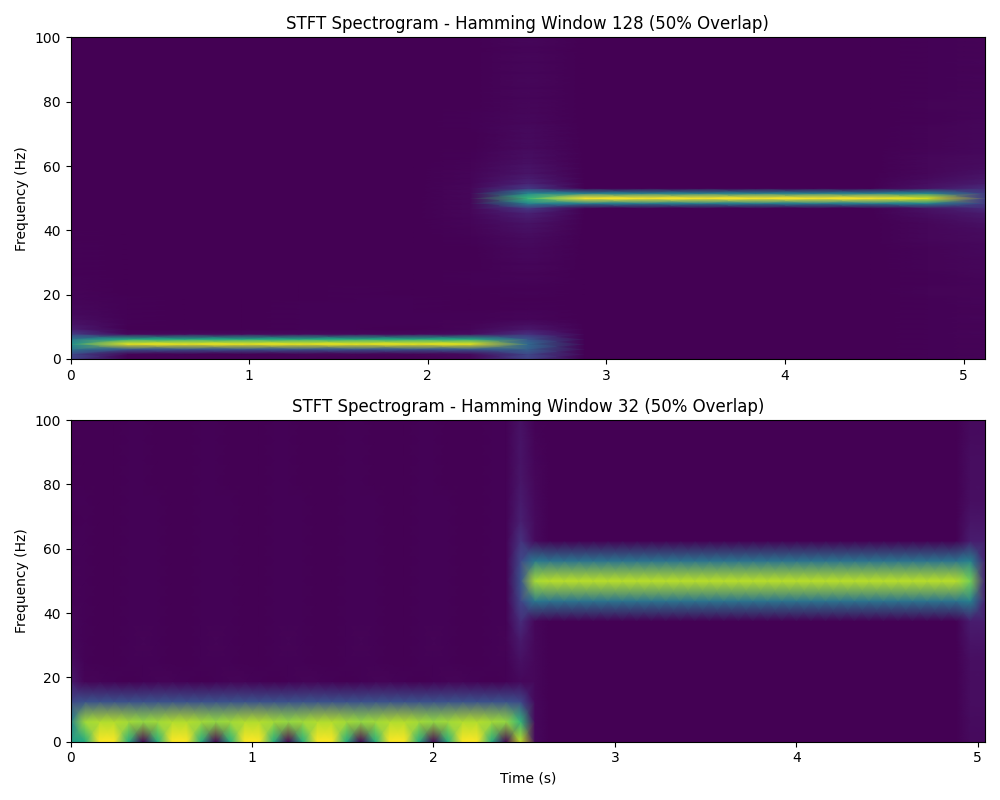
\includegraphics[width=0.8\textwidth]{plots/spectrograms.png}
    \caption{STFT Spectrogram Comparisons for varying Window sizes.}
\end{figure}

\subsection{Comparison and Review}
\begin{itemize}
    \item \textbf{Window 128 (Top Plot):} The time transition presents mild horizontal latency mapping across boundaries. The frequencies, however, are \textit{very definitively separated} onto specific narrow horizontal bands.
    \item \textbf{Window 32 (Bottom Plot):} The temporal localization of the frequency transition occurring exactly at 2.5 seconds is visibly sharper with much fewer intermediary blocks. Conversely, the strict frequency bands are now severely smeared vertically along the Y-axis.
    \item \textbf{Projection ($N=256, 512$):} Should an extremely extended window ($N=256$ or $512$) be applied, the frequency resolution would theoretically collapse to practically impulse lines. However, detecting the temporal disruption timestamp would be nearly impossible, smearing transition artifacts across large fractional spans ($> 50\%$) of the recording.
\end{itemize}

\end{document}
